\documentclass[a4paper,twoside,12pt]{report}
% Marcell Nagy (2022)

% Include Packages
\usepackage[a4paper,inner=3.5cm,outer=2.5cm,top=2.5cm,bottom=2.5cm]{geometry}  % Set page margins
\usepackage{fullpage}
\usepackage{float}                  % Allows 'Here and Only Here' [H] for Floats
\usepackage{url}                    % \url{} command
\usepackage{charter}            	 % Set font to Times
\usepackage{graphicx}               % \includegraphics
\usepackage{subfig}              	 % Allow subfigures
\usepackage{amsmath}
\usepackage{color}
\usepackage{tikz}
\usepackage[all]{nowidow}
\usepackage{enumitem}
\usepackage{datenumber}
\usepackage{amsthm}
\usepackage{amssymb}
\usepackage{booktabs}
\usepackage{parskip}
\usepackage{pgfgantt}
\setnoclub[2]
\setnowidow[2]

% Referencing
% Provides \Vref and \vref to indicate where a reference is.
\usepackage{varioref} 
% Hyperlinks references
\usepackage[bookmarks=true,bookmarksopen=true]{hyperref} 
% Provides \Cref, \cref, \Vref, \vref to include the type of reference: fig/eqn/tbl
\usepackage{cleveref} 
% Setup Hyperref
\hypersetup{
  colorlinks   = true,              %Colours links instead of ugly boxes
  urlcolor     = blue,              %Colour for external hyperlinks
  linkcolor    = blue,              %Colour of internal links
  citecolor    = blue               %Colour of citations
}
% Names for Clever Ref
\crefname{table}{table}{tables}
\Crefname{table}{Table}{Tables}
\crefname{figure}{figure}{figures}
\Crefname{figure}{Figure}{Figures}
\crefname{equation}{equation}{equations}
\Crefname{equation}{Equation}{Equations}

% Wits Citation Style
\usepackage{natbib} % Force natbib.sty to put citation labels in the reference list
\makeatletter
\renewcommand\NAT@biblabel[1]{\def\citeauthoryear##1##2{##1 ##2}[#1]\hfill}
\renewcommand\NAT@bibsetup[1]{%
  \setlength{\itemsep}{\bibsep}\setlength{\parsep}{\z@}}
\def\@lbibitem[#1]#2{%
  \if\relax\@extra@b@citeb\relax\else
    \@ifundefined{br@#2\@extra@b@citeb}{}{%
     \@namedef{br@#2}{\@nameuse{br@#2\@extra@b@citeb}}}\fi
   \@ifundefined{b@#2\@extra@b@citeb}{\def\NAT@num{}}{\NAT@parse{#2}}%
   \item[\hfil\hyper@natanchorstart{#2\@extra@b@citeb}\@biblabel{#1}%
    \hyper@natanchorend]%
    \NAT@ifcmd#1(@)(@)\@nil{#2}}
\makeatother


\bibliographystyle{named-wits}
\bibpunct{[}{]}{;}{a}{}{}  % to get correct punctuation for bibliography
\setlength{\skip\footins}{1.5cm}
\newcommand{\citets}[1]{\citeauthor{#1}'s \citeyearpar{#1}}
\renewcommand\bibname{References}  

\pagestyle{headings}

\pagestyle{plain}
\pagenumbering{roman}

\renewenvironment{abstract}{\ \vfill\begin{center}\textbf{Abstract}\end{center}\addcontentsline{toc}{section}{Abstract}}{\vfill\vfill\newpage}
\newenvironment{declaration}{\ \vfill\begin{center}\textbf{Declaration}\end{center}\addcontentsline{toc}{section}{Declaration}}{\vfill\vfill\newpage}
\newenvironment{acknowledgements}{\ \vfill\begin{center}\textbf{Acknowledgements}\end{center}\addcontentsline{toc}{section}{Acknowledgements}}{\vfill\vfill\newpage}

\setlist[itemize]{noitemsep}

\begin{document}
\onecolumn
\thispagestyle{empty}

\setcounter{page}{0}
\addcontentsline{toc}{chapter}{Preface}
\ 
%%%%%%%%%%%%%%%%%%%%%%%%%%%%%%%%%%%%%%%%%%%%%%%%%%%%%%%%%%%%%%%%%%%%%%%%%%%%%%%%%%%%%%%%%%%%%%%%
\begin{center}
  \vfill
  {
  \huge \bf \textsc{Ball tracking by object detection}\\
  \large using deep neural network aided Kalman filtering in a\\
  \large real-time simulated RoboCup Soccer environment\\[20pt]
  \large School of Computer Science \& Applied Mathematics\\
  \large University of the Witwatersrand\\[20pt]
  \normalsize
  Marcell Nagy\\
  2628829\\[20pt]
  Supervised by Prof. Richard Klein \\
  and Dr. Pravesh Ranchod\\[10pt]
  \today
  }
  \vfill
  \vfill
  
\includegraphics[width=1.5cm]{images/wits}
  \vspace{10pt}\\
%  \small{Ethics Clearance Number: XX/XX/XX}\\[10pt]
  \small{A research report submitted to the Faculty of Science, University of the Witwatersrand, Johannesburg,
in partial fulfillment of the requirements for the degree of Master of Science}\\
\end{center}
\vfill

\newpage
\pagestyle{plain}
\setcounter{page}{1}

%%%%%%%%%%%%%%%%%%%%%%%%%%%%%%%%%%%%%%%%%%%%%%%%%%%%%%%%%%%%%%%%%%%%%%%%%%%%%%%%%%%%%%%%%%%%%%%%
\phantomsection
\begin{abstract}
Computer vision has the ability provide an abundance of environmental information to a robotic system, which makes perception and interaction with a dynamic world possible. In this research report, the problem of real-time ball tracking in the context of simulated RoboCup soccer is considered. A tracking-by-detection framework is utilized, to take advantage of the high performance of modern neural detection techniques, as well as the use of neural assisted Kalman filtering for tracking, which strikes a balance between the ease of interpretation of the traditional model-based approach and the ability to learn complex dynamics using neural networks. The results show that a modern key point based detector can outperform both  traditional Viola Jones based detection as well as popular anchor based detection approaches in the context of simulated robocup soccer. Further, a neural approach to Kalman filtering is able to outperform the popular extended Kalman filter for simulated robocup soccer kick tracking. 

\end{abstract}

%%%%%%%%%%%%%%%%%%%%%%%%%%%%%%%%%%%%%%%%%%%%%%%%%%%%%%%%%%%%%%%%%%%%%%%%%%%%%%%%%%%%%%%%%%%%%%%%
\phantomsection
\begin{declaration}
I, Marcell Nagy, hereby uniquely declare the contents of this research report to be by my own efforts.
This research report is prepared for the degree of Master of Science (Robotics) at the University of the Witwatersrand.
This material has not been submitted to any other university, or for any other degree.
\end{declaration}

%%%%%%%%%%%%%%%%%%%%%%%%%%%%%%%%%%%%%%%%%%%%%%%%%%%%%%%%%%%%%%%%%%%%%%%%%%%%%%%%%%%%%%%%%%%%%%%%
\phantomsection
\begin{acknowledgements}
Thank you Prof. Richard Klein and Dr. Pravesh Ranchod for your constructive comments, feedback and support throughout my studies. I'm inspired by your unfailing willingness to go out of your way to help students. Your enthusiasm for computer science is contagious.
\end{acknowledgements}

%%%%%%%%%%%%%%%%%%%%%%%%%%%%%%%%%%%%%%%%%%%%%%%%%%%%%%%%%%%%%%%%%%%%%%%%%%%%%%%%%%%%%%%%%%%%%%%%
\phantomsection
\addcontentsline{toc}{section}{Table of Contents}
\tableofcontents
\newpage
\phantomsection
\addcontentsline{toc}{section}{List of Figures}

%%%%%%%%%%%%%%%%%%%%%%%%%%%%%%%%%%%%%%%%%%%%%%%%%%%%%%%%%%%%%%%%%%%%%%%%%%%%%%%%%%%%%%%%%%%%%%%%
\listoffigures
\newpage
\phantomsection
\addcontentsline{toc}{section}{List of Tables}

%%%%%%%%%%%%%%%%%%%%%%%%%%%%%%%%%%%%%%%%%%%%%%%%%%%%%%%%%%%%%%%%%%%%%%%%%%%%%%%%%%%%%%%%%%%%%%%%
\listoftables
\newpage
\pagenumbering{arabic}

%%%%%%%%%%%%%%%%%%%%%%%%%%%%%%%%%%%%%%%%%%%%%%%%%%%%%%%%%%%%%%%%%%%%%%%%%%%%%%%%%%%%%%%%%%%%%%%%
\chapter{Introduction}

Object tracking is an important practical topic in the domain of robotics. The ability of an agent to identify, localize and capture the trajectories of objects is an essential task required for perception of and interaction with a dynamic environment. A variety of methods are possible for capturing the state information of a target object -- with some examples being: mechanical trackers which consists of sensorised linkages connecting an object to a frame of reference, inertial trackers such as accelerometers which measure the rate of change of velocity as well as vision based systems that optically capture a scene and use processing to extract relevant information \citep{track2}. Compared to techniques which measure the object state directly, vision can capture vast additional information such as multiple objects, position, pose,  and context as well being versatile in a sense that it does not intrinsically depend on material properties or addition of sensors to a tracked object. However, extracting information accurately with real-time performance using a computationally and memory constrained device remains an inherit challenge in robotics \citep{quantization, kalmannet}. 

Modern computer vision is dominated by deep learning approaches. Traditional computer vision utilizes pipelines with hand-crafted feature extractors and shallow machine learning algorithms to perform classification and regression tasks. The effectiveness of deep learning techniques over traditional techniques results from the ability to rather learn feature extraction from training data as well as introducing end-to-end learning which reduces the multi-staged pipeline and allows a more encompassing optimization \citep{tradvmod}. Traditional approaches are still useful in certain contexts, typically providing intuitive solutions and requiring less data, memory and training time.

More formally, in visual object tracking, the aim is to use a sequence of image frames to robustly estimate the motion state of a target object \citep{track1}. Many different visual object tracking paradigms are possible, with some popular traditional approaches being tracking-by-detection, optical flow, silhouette tracking or discriminative correlation filters to name a few \citep{track0}. During initialization of any object tracker -- unless manually targeted -- objects must first be selected using an object detector \citep{tradtrack0}. One might question then, why not just use object detection on each frame to track an object? According to \cite{tradtrack5} \textit{``tracking is easier than detection, tracking algorithms can use fewer computational resources than running an object detector on every frame''}. Modern approaches to tracking include applying CNN feature extraction to traditional tracking frameworks and end-to-end deep learning where a variety of network architectures have been used including convolutional neural networks (CNN), siamese neural networks (SNN), recurrent neural networks (RNN) and generative adversial networks (GAN) as some examples \citep{deeptrack1}. With the advancement of modern object detection methods for real-time implementation, such as You Only Look Once (YOLO) by \cite{yolo} for example, it becomes interesting to apply these effective models to a tracking-by-detection framework. According to \cite{deepsort}, this approach has become the leading paradigm for object tracking.

Object detection is a computer vision task where objects are identified (classification) and localised in an image (regression). From a single frame it is possible to determine position (and other states such as pose), however, without establishing correspondence within an image sequence time-dependent states such as velocity cannot be computed and the state estimate lacks robustness. Here robustness means that noise such as misclassification is attenuated as well as providing instance identification and resilience to occlusion. These can be achieved by linking the frames of the image sequence (also known as data association). \cite{tradtrack0} states that \textit{``The simplest method to perform correspondence is to use the nearest neighbor approach. However, if the objects are close to each other, then there is always a chance that the correspondence is incorrect''}.

A downside of deep learning approaches is that they demand a significant amount of training data in order to achieve useful results. Accurately labeled real world training images come at a labour cost, which makes the use of a simulated environment an efficient choice. This approach is still practical to application  in the real world, advances in domain adaptation have shown significant success in mapping a simulated environment to a physical environment \citep{domainadpt}. Additionally, photo realistic rendering can also be applied \citep{sim4cv}. These topics will however not be investigated in this research. In this research, visual ball tracking will be investigated in the context of 3D simulated RoboCup soccer, which is an international robotics competition  that has been entered by the Robotics, Autonomous Intelligence and Learning (RAIL) Lab from the School of Computer Science and Applied Mathematics at the University of the Witwatersrand \citep{witsfc}. Although the current focus of the team is the 3D simulation league, physical leagues are in consideration for the future. 

\section{Structure}

The research report continues as follows. Firstly in the introductory chapters, a background section is presented (Chapter 2) which gives relevant context with regards to the research problem and the chosen techniques. This is followed by a related work section (Chapter 3) which presents a selection of published work, in a similar problem space, where some of the important methods and results that are considered in this work are summarized. Then, the research problem is outlined (Chapter 4) prior to presenting the research methodology (Chapter 5). Continuing to the central chapters, the investigations focusing on object detection (Chapter 6) and object tracking (Chapter 7) are presented respectively. Finally, a concluding chapter is given (Chapter 8).

%%%%%%%%%%%%%%%%%%%%%%%%%%%%%%%%%%%%%%%%%%%%%%%%%%%%%%%%%%%%%%%%%%%%%%%%%%%%%%%%%%%%%%%%%%%%%%%%
\chapter{Background}

In this section, an overview is given for some of the underlying topics relevant to ball tracking. Firstly, the object tracking problem is considered (Section 2.1). It is found that a tracking-by-detection approach can be used to produce state-of-the-art results by taking advantage of the progress made in the popular object detection problem space. Further, the intuitive Kalman filtering algorithm is found to still be relevant in the modern tracking context and a recent approach to improve its results for complex systems by incorporating a neural-based step is discussed. Following on, the object detection problem is considered  (Section 2.2) and some of the modern approaches and progress is addressed. The context of RoboCup Soccer is introduced (Section 2.3).

\section{Object tracking}

Object tracking describes the problem of estimating the trajectory of an object as it moves around the scene. Object tracking can be divided into offline (also known as batch) and online problem spaces. In the offline problem a complete image sequence can be used, whereas in online problems only the images of the previous time steps are available  \citep{track0}. Real-time tracking is online by definition. Some of the challenges include object occlusion, objects going out of frame, complex object motion, background clutter, dynamic backgrounds, imaging noise, motion blurring, illumination changes, object deformation, multiple instances, monocular vision and real time processing requirements \citep{tradtrack0}.

An object tracker can be understood using the general framework suggested by \cite{diagnosingtrack} where the authors have decomposed and studied the object tracking problem in its constituent parts. Figure \ref{fig:tracker} provides a representation of a generalized tracking process. Here it is assumed that an ensemble model is not utilized, which is typically avoided for real time application due to a higher computational demand. The modeling of the object motion and appearance aids with data association as well as improving trajectory estimation. \citep{sort}  

\begin{figure}[h!]
\begin{center}
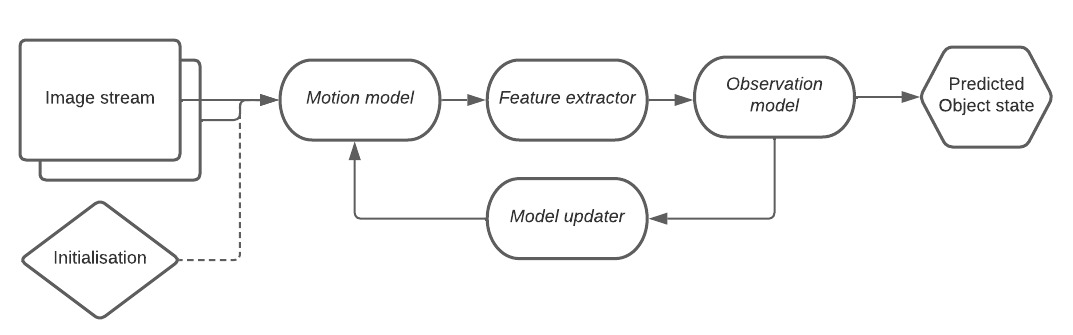
\includegraphics[width=13.5cm]{images/Tracking_flowchart.jpeg}
\caption{Generalized tracker flowchart}
\label{fig:tracker}
\end{center}
\end{figure}

\pagebreak
The components are described as follows:

\begin{itemize}
    \item Initialization -- An object to be tracked is selected manually or by detection.
    \item Motion model -- Generates candidates that may contain the tracked object.
    \item Feature extractor -- Acquires a representation of the objects in the image.
    \item Observation model -- Classify if is the tracked object. Assigns detection to target.
    \item Model Updater -- Adaptation of the observation model.
\end{itemize}

It is reported that not all components have equal importance, which is useful insight when real-time performance is desired. \cite{diagnosingtrack} conclude, \textit{``Contrary to popular belief, it turns out that the observation model (which is the focus of many papers on visual tracking) does not play the most important role in a tracker''}. Feature extraction is found to affect the performance most - which is a task that CNNs excel at. An object tracker which utilities the progress of CNN detection methods is a popular algorithm: ``Simple Online and Realtime tracking'' (SORT) \citep{sort}.

\subsection{SORT}

SORT is a visual object tracking technique which is based on the Kalman filter \citep{kalman} and Hungarian method \citep{hungarian}. A Kalman filter is a recursive state estimator which fuses a motion model and measurement to predict the motion state of a linear system \citep{trackbook}. 

\subsubsection{Kalman filtering}

In this model, object motion is described by a discrete linear time invariant (LTI) state-space process which defines the evolution of the state from time $t-1$ to time $t$ as:
\begin{equation} 
x_t=Fx_{t-1}+Bu_{t}+w_{t}
\end{equation}
Where $x_{t}$ is the object state at time $t$ of ($n \times 1$) shape, $F$ is the state transition matrix (from a system dynamics model) of ($n \times n$) shape which describes how the state evolves between time $t$ and $t-1$. $B$ is the control-input matrix and $u$ the control vector which models the effect of control signals into the system. $w$ is the process noise vector which is normally distributed about a mean of zero with variance $Q$ which accounts for neglected and uncertain modeled behavior.

An observation model describes the relationship between the object state and the measurement at the current time step:
\begin{equation} 
z_t=Hx_{t}+{\upsilon}_t
\end{equation}
Where $z_{t}$ is the measurement vector at time $t$ of ($m \times 1$) shape, $H$ is the measurement matrix of ($m \times n$) shape which maps measurements to the object state. $\upsilon$ is the measurement noise vector which is normally distributed about a mean of zero with variance $R$ which accounts for measurement uncertainty.

The Kalman filtering algorithm is then performed for state estimation as follows. The ``prediction step'' is computed as:
\begin{equation}
\hat{x}_{t|t-1}=F\hat{x}_{t-1|t-1}+Bu_{t|t}
\end{equation}
\begin{equation}
\hat{P}_{t|t-1}=F\hat{P}_{t-1|t-1}F^T+Q 
\end{equation}
Where $\hat{x}_{t|t-1}$ and $\hat{P}_{t|t-1}$ are the state and the covariance predictions at  time $t$. $Q$ is the process error covariance.

The ``correction step'' is then computed as:
\begin{equation} 
K = \hat{P}_{t|t-1}H^T(H\hat{P}_{t|t-1}H^T+R)^{-1}
\end{equation}
\begin{equation} 
\hat{x}_{t|t} = \hat{x}_{t|t-1}+K(z_t-H\hat{x}_{t|t-1})
\end{equation}
\begin{equation} 
\hat{P}_{t|t}=(I-KH)\hat{P}_{t|t-1}
\end{equation}
$K$ is known as the Kalman gain which, for linear systems with gaussian noise, can be optimally computed for mean-square error to apply a correction based on the relative uncertainty between the process and measurement. This can be understood as a trade-off between the model predicted state and the measurement. In typical usage, $\hat{P}_0$ is initialized to a relatively high value which has the impact of the system largely ignoring the assigned value of $\hat{x}_{0}$ in favor of the first measured state.

In the case of a nonlinear state transition or measurement mapping, object motion can be modeled more generally by:
\begin{equation} 
x_t=f(x_{t-1},u_{t})+w_{t}
\end{equation}
\begin{equation} 
z_t=h(x_{t})+{\upsilon}_t
\end{equation}
Systems with nonlinear state transition or measurement mappings can be linearized at each time step, using the Taylor series expansion, and used in the standard equations to obtain the Extended Kalman Filter (EKF) \citep{trackbook}. The resulting matrices can each be described as Jacobians respectively (first-order partial derivatives):
\begin{equation}
F_t = \frac{\partial f(\mu_{t-1}, u_{t})}{\partial x_{t-1}}
\end{equation}
\begin{equation} 
H_t = \frac{\partial h(\mu_{t})}{\partial x_t} 
\end{equation}
 $\mu$ refers to the state about which the linearization occurs. The EKF is non-optimal however remains powerful and is popularly applied.

\subsubsection{SORT algorithm}

With real-time performance being a crucial component of online tracking, the light weight and minimalist nature of the SORT algorithm supports rapid update cycles. Despite its simplicity, it performs exceptionally well. \cite{sort} state, \textit{``This approach achieves an accuracy comparable to state-of-the-art online trackers.''} Furthermore, due to the computational simplicity of their method, the algorithm achieves a rapid update rate of 260 Hz which is quoted to be over 20x faster than other state-of-the-art trackers and certainly exceeding real-time requirements.

SORT comprises of the following components:
\begin{itemize}
	\item A linear constant velocity model which is used to model the states of a tracked object. Without a detection associated to the object, its state is simply predicted without correction using the linear velocity model. With an associated detection, the predicted bounding box can be used to update the object states using the Kalman filtering algorithm.

	The state of each object is modelled as:
\begin{equation}
x = [u,v,s,r,\dot{u},\dot{v},\dot{s}]^T
\end{equation}
With u and v representing the horizontal and vertical location of the center of the object and the area (s) and aspect ratio (r) of the target’s bounding box.

	\item For feature extraction, the original implementation uses an object detector known as ``Faster R-CNN'', however, since SORT utilities only bounding box position and size for both motion estimation and data association \citep{sort} it is possible to evaluate and choose any sufficiently performing object detector.
	\item To assign detections, each object's new bounding box is predicted. The IoU score (see object detection) is then computed between each detection and all predicted bounding boxes and the association problem is then solved optimally using the Hungarian algorithm.
\end{itemize}

\cite{sort} reiterate the strong influence of object detector performance on overall tracking results. Further, the relevance of the Kalman filter is reaffirmed in modern tracking applications. More recent work by \cite{sort++} shows that a constant velocity model with a Kalman filter and Hungarian method is still a powerful tracking approach. For robotics applications, SORT trackers are still \textit{``achieving state-of-the-art results with a high frame rate''} \citep{sortrob}.

\subsection{Deep SORT}

As an extension to the SORT algorithm, Deep SORT (Simple Online and Realtime Tracking With a Deep Association Metric) has been introduced by \cite{deepsort}. In this extension, appearance information is included into the observation model in an attempt to improve the performance for multiple objects. The addition is effective at reducing the number of identity switches, which permits longer periods of occlusions, however, it comes at a cost of real-time performance. Therefore in the case of real-time single object tracking, it does not provide sufficient benefits over SORT. 

\pagebreak
\subsection{KalmanNet}

The Kalman filter remains an effective and relevant tracking algorithm which finds itself in common use in computer vision and robotics \citep{kalmanforever}. A downside of model based methods is that performance relies on accurate knowledge of the underlying dynamics -- which typically requires domain knowledge and valid assumptions. Modern data driven approaches try to learn entirely from data, however, they have many parameters, require significant amounts of data and lack intuition, which prevents their application in embedded systems \citep{kalmannet}.

\cite{kalmannet} propose a hybrid data-driven and model based approach to real-time Kalman filtering, where the underlying state space model is non-linear and accurate knowledge of it is unknown. In this approach a recurrent neural network (RNN) (more specifically a Gated Recurrent Unit (GRU) variant) can be trained on representative data in order to predict the appropriate Kalman gain at each time step  (See figure \ref{fig:blockd}). Compared to ``traditional'' feed-forward neural networks where fixed length input data simply flows through the network to compute an output, in an RNN the input as well as a hidden state (which represents the history) are fed back into the network -- which allows a series of temporal information to be processed  (See figure \ref{fig:architecture}). 

\begin{figure}[h!]
\begin{center}
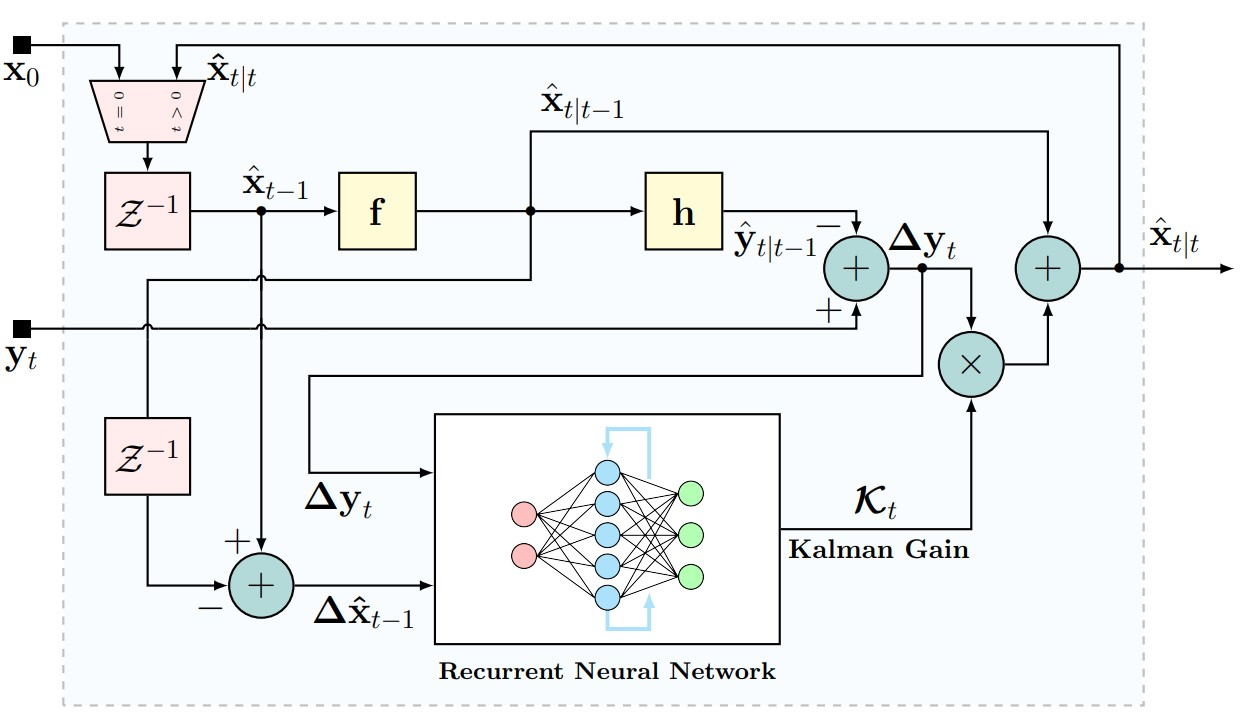
\includegraphics[width=12.5cm]{images/kalmannet1.jpg}
\caption{KalmanNet block diagram \citep{kalmannet}}
\label{fig:blockd}
\end{center}
\end{figure}

\begin{figure}[h!]
\begin{center}
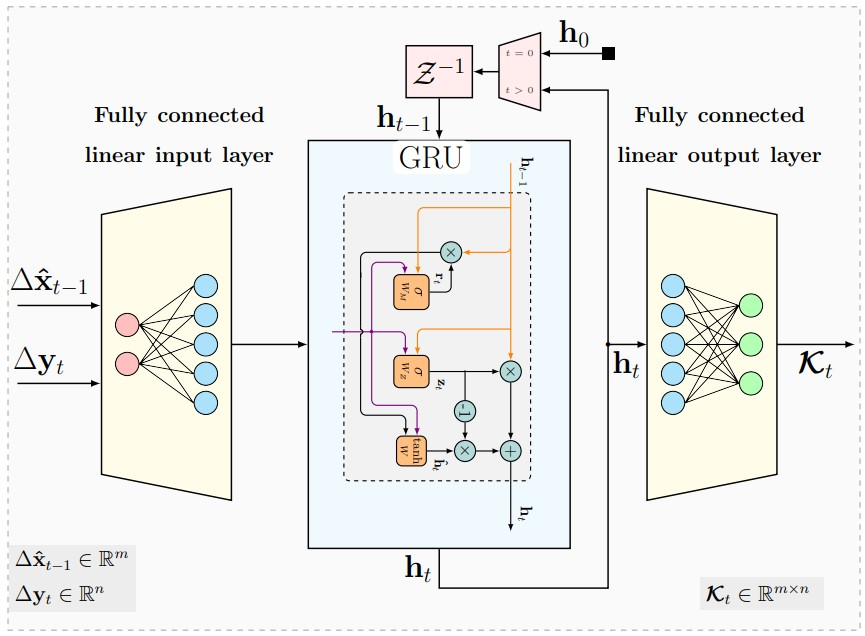
\includegraphics[width=10cm]{images/kalmannet2.jpg}
\caption{KalmanNet RNN \citep{kalmannet}}
\label{fig:architecture}
\end{center}
\end{figure}

In this manner, KalmanNet removes the dependency of knowledge of the underlying process and measurement noise and a facilitates a partially known or approximated underlying state space model from a system dynamics model.

The interpretability of the original algorithm is retained whilst implicitly learning complex dynamics, reducing the need for domain knowledge and model assumptions that are needed to accurately characterize a complex system as a tractable state space model. \cite{kalmannet} conclude, \textit{``KalmanNet is shown to converge much faster compared with purely DD (data driven) systems, while outperforming the MB (model based) EKF (extended Kalman filter), UKF (Unscented Kalman filter), and PF (particle filter), when facing model mismatch and dominant non-linearities''}. This data driven approach to Kalman filtering has recently found other robotics applications -- replacing the extended Kalman filter for online Simultaneous localization and mapping (SLAM) -- a crucial task for robotic systems where a map of an environment is simultaneously constructed while localizing the position of an agent \citep{slam}.

\subsection{Performance measures}

A useful performance measure used for evaluating state estimators is the Root Mean Square Error (RMSE) -- which can be considered as the standard deviation of the difference between the predicted state and the ground truth. \citep{kalmanperform}

RMSE can be computed as follows:
\begin{equation}
RMSE = \sqrt{\frac{1}{M}\sum^{M}_{i=1}\epsilon_{i}^{2}}
\end{equation}

Where $\epsilon_{i}$ is the error for the $i$th sample which is difference between the predicted and ground truth state. RMSE is often used as a statistical design criterion for noisy systems as it prescribes a soft bounds based on probability (for true Gaussian noise it is by definition that 99.7\% of samples will occur within three standard deviations).

\newpage
\section{Object detection}

Object detection is one of the oldest and well studied computer vision problems. Within the scope of this problem is facial recognition, pedestrian recognition and multi-class classification which have historically received significant attention in various competitions and the establishment of various  datasets such as Caltech pedestrians \citep{peddetect}, PascalVOC \citep{vocdataset} and Microsoft COCO \citep{coco}.

\subsection{Traditional Object detection}

With the most successful approaches being based on discriminative models -- a traditional object detector can be considered in general to have the following components:  Region selection, feature extraction and classification \citep{deepreview}:

\begin{itemize}
    \item In region selection, different sub windows are considered at various scales and are passed into the detector window. This may be by a region proposal algorithm or by scanning the entire image at different scales. This approach is less complex than processing the entire image and allows a single detector to be trained and applied throughout the image, but is computationally expensive. 
    \item Feature extraction attempts to capture patterns in the image that represent an object or provide semantic information. Low level features (textures, edges, etc.) may be combined with spacial information into a single feature descriptor.
    \item A classifier predicts the presence of an object class in the window given the extracted features. The decision boundary (which is an $n-1$ dimensional surface in an $n$ dimensional domain) is learnt using training examples. For a positive detection, the current window is returned as a bounding box. Since multiple windows will return positive for the same object, techniques such as non maximum suppression can be used to isolate a single prediction.
\end{itemize}

\noindent Some of the criticisms of traditional strategies are: 
\begin{itemize}
    \setlength\itemsep{0em}
    \item Generating bounding boxes with a sliding window strategy is inefficient and inaccurate
    \item Using hand crafted low level features it is difficult to adequately capture the semantics of the image 
\end{itemize}

Traditional object detectors that had relative success and some real-time application include the Viola Jones algorithm \citep{vjdet} as well as the HOG features and SVM classification based D\&T detector \citep{hog}. 

\subsubsection{Viola Jones detection}

The Viola Jones (VJ) detector \cite{vjdet} was a breakthrough algorithm that was considered to be the first viable real time object detector still maintaining state-of-the-art accuracy. Although targeting face detection, it can be equally applied to different object classes. The VJ detector uses a sliding window detector with a fixed step size. A scaling factor can be applied to the window which increases the filter size proportionally after each complete image traversal in order to search for larger faces. 

Firstly considering feature extraction, an observation can be made that classes of objects, such as faces, have a typical layout that can be approximated by patterns of adjacent lighter and darker regions. ``Haar-like'' features (Figure \ref{fig:haarft}) are applied to a gray-scale image to capture the differences in regions with a single number. Filters of pattern A and B respond to edges, filters of pattern C respond to lines and filters of pattern D respond to diagonal features. During training, an exhaustive search for features is performed where all possible scale, aspect ratios and positions of the filters in the detection window are considered for each training face example - a base resolution of 24x24 for the window is used which gives approximately 180k features for each detection window. 

\begin{figure}[h!]
    \centering
    \subfloat{{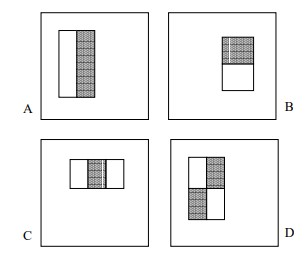
\includegraphics[height=5cm]{images/haarft.jpg}}\label{fig:haarft}}
    \qquad
    \subfloat{{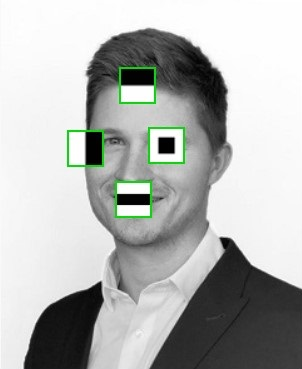
\includegraphics[height=5cm]{images/vjtest.jpg}}}
    \caption{Haar features \cite{vjdet} (Left) and strong responses (Right)}
\end{figure}

\citeauthor{vjdet} (\citeyear{vjdet}) introduce an elegant approach to evaluate these features rapidly by precomputing an intermediate ``integral image'' which allows the subsequent computation of a region in constant time. 

In order to classify each window, there are a significant number of Haar-like features possible at each possible detection. An efficient approach to classification, based on the adaBoost machine learning algorithm, is used as a ``feature selection'' process by training and selecting a subset of weak classifiers that can be combined into a strong classifier. The set of ``cascading classifiers'' are arranged as a degenerate decision tree, where each node is a stage of increasing complexity. False classifications cause an early exit from the cascade, therefore background regions are rejected quickly and more computation is spent on distinguishing complex regions. The speed of processing an image is therefore impacted by the complexity of the image. Using less stages and features can result in faster compute times. Faster speeds can also be achieved by increasing the step sizes and scaling factor.

\newpage
\subsection{Modern Object detection}

Before the dramatic growth and change of focus towards modern computer vision techniques, traditional object detectors were reaching saturation. \citep{rcnn} echo this sentiment: \textit{``Object detection performance, as measured on the canonical PASCAL VOC dataset, has plateaued in the last few years. The best-performing methods are complex ensemble systems that typically combine multiple low-level image features with high-level context''}.

Deep learning approaches are considered to have become the state of the art since the year 2012 with AlexNet becoming the first CNN to lead the ImageNet Large Scale Visual Recognition Challenge (ILSVRC) \citep{alexnet}. The first widely popularized object detector to make use of CNNs is R-CNN (Regions with CNN features) \citep{rcnn}, which uses CNNs for feature extraction but otherwise retains a traditional detector pipeline with region proposal. CNN based detectors which utilize a region proposal stage and are known as two-stage detectors \citep{comprehensive}.  Modern object detectors are able to achieve near perfect results on data-sets that traditional architectures fail to show even marginal comprehension of. This can be seen in the benchmarking of the You Only Look Once (YOLO) object detector (See figure \ref{fig:yoloplot}) \citep{yolo} versus the D\&T detector of \cite{hog}.

\begin{figure}[h!]
\begin{center}
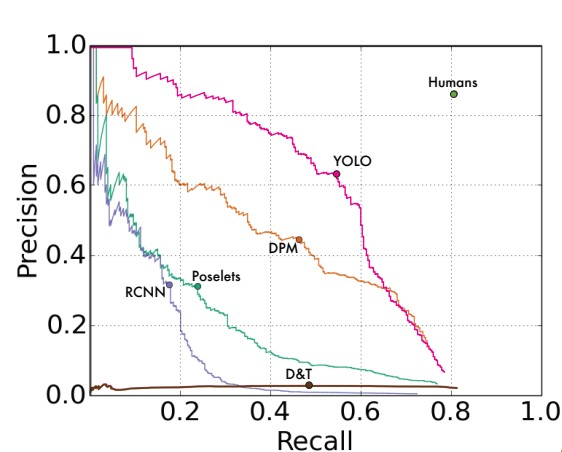
\includegraphics[width=8.5cm]{images/yoloplot.jpg}
\caption{YOLO precision-recall curve \citep{yolo}}
\label{fig:yoloplot}
\end{center}
\end{figure}

Modern object detectors utilize deep CNNs in order to learn feature extraction. CNNs are based upon the mathematical operation of convolution, where a matrix called a filter kernel is swept across an image in order to take advantage of the spacial context of an image. CNNs are able to extract both low level and high level contextual features due to a hierarchical network structure, often referred to as the backbone of the network. The networks can be trained by minimizing a loss function that combines the regression and classification performances. The object detection problem can be considered as the combination of both classification and regression tasks. A loss function is a measure of the algorithm error for the considered task and the aim of training is to find a local minimum of this objective. 

Categorical cross-entropy loss is a popular choice for classification tasks, when categorical variables are considered, as it is readily differentiable for back-propagation:

\begin{equation}
L_{classification} = -\sum_{i=1}^{n}t_i log(p_i)
\end{equation} 
With $t_i$ being the ground-truth and $p_i$ being the softmax probability for the $i_{th}$ class.

Least square error ($L_2$ loss) is a common choice for regression loss when considering continuous variables:
\begin{equation}
L_{regression} = \sum(y_i-\hat{y_i})^2 
\end{equation} 
Where $y_i$ is the ground truth.

\subsubsection{YOLO}

A breakthrough for object detection was achieved with the introduction of the one-stage detector YOLO by \cite{yolo} which achieved real-time speeds whilst remaining competitive with state-of-the-art detectors. The speed of single stage detectors is in general considered to be faster than that of two-stage detectors -- but at a cost of accuracy. According to \cite{stagecomp} regarding two stage detection: \textit{``This architecture can achieve more reliable detections, but increases the required computation, hence being less convenient for real-time applications''}. In the YOLO architecture, various predefined ``anchor'' boxes are placed and evaluated - which is known as an anchor based approach. As per \cite{yolo} some disadvantages of this approach is that the detector is sensitive to these hyper-parameters and has difficulty detecting objects much smaller than the anchors as well as suffering from some localisation error: \textit{``While it can quickly identify objects in images it struggles to precisely localize some objects, especially small ones''}.

Many variations of the YOLO algorithm exist, where most do not originate from or have any permissions from the original researchers. In the classic YOLO architecture, the image is divided into grid cells of $S\times S$ (typically $13\times 13$ is used) - which is achieved by down-sampling with the convolutional backbone. For each cell, predefined bounding boxes (with $B$ number of boxes per cell - 5 is typical) are used as initial guesses for object location and size - which drives the depth of the feature map. These box dimensions are learnt via using k-means clustering on the training data (thereafter referred to as dimensional priors). For each anchor box, we predict class and objectness (probability of an object in the given region). For localisation, offsets from the prior is then predicted. A small localisation improvement can be gained by including a lower level feature map with higher resolution using a pass-through layer, which is concatenated with the grid representation using a "reorganisation" layer. \citep{comprehensive}

To train the network, a multipart loss is optimised. The function has the following high level form:
\begin{equation}
L_{YOLO} =  \lambda L_{reg} + L_{confi} + L_{cls} 
\end{equation} 
With $\lambda$ as a balancing weight for training emphasis.

\subsubsection{NanoDet}

Contemporary object detection advancements include anchor box free detectors -- which reformulate the problem as keypoint detection. This frees the detector from the anchor box hyperparameters such as size and aspect ratio as well as allowing for simpler architecture which allow for faster computation. Although CornerNet \citep{cornernet} was proposed as the first alternative to the single stage anchor-based approaches, more recent state-of-the-art models include Fully Convolutional One-stage Object Detection (FCOS) \citep{fcos} and the subsequent NanoDet \citep{nanodet} which has been shown to be the current state-of-the-art for real-time obejct detection as shown by the comprehensive study of \cite{comprehensive}. In a keypoint based approach, a convolutional neural network is used to predict heatmaps, with the intensity peaks representing corners or object centers. The dimensions of the  bounding boxes are then predicted. \cite{comprehensive} report: \textit{``The keypoint-based methods generally outperform the anchor-based and two-stage methods in terms of accuracy and speed''} 

Anchor-free object detectors utilise key-points (such as centers and corners of objects) rather than anchors to perform regression from. A benefit of this approach is that it eliminates the anchor-box hyper-parameters, which are particularly dataset-dependant, as well as avoiding the problem of having to compute and reject redundant (non-maximal) box predictions. According to \cite{cnet} \textit{``Most successful object detectors enumerate a nearly exhaustive list of potential object locations and classify each. This is wasteful, inefficient, and requires additional post-processing.''}  

In the ``FCOS-style'' key-point approach which NanoDet is based on, each object is modelled as a single center point of a bounding box. The idea is that an input image is processed into a heat-map image where the highest activation values occur at the object center with a different channel for each class. Bounding box dimensions are then regressed from this point. 

In the pipeline, after feature extraction, up-sampling is performed to create a higher-resolution output to incorporate more spacial detail - the resolution used is 4 times less (called output stride $R$) than the input image resolution.

A single network is then used to predict key-point, size and offsets: 
\begin{itemize}
    \setlength\itemsep{0em}
    \item \textbf{Classification} - This branch outputs a heat-map to estimate the center points of the objects. The number of heat-maps is equal to the number of classes. For multi-scale training, non-maxima suppression is performed to merge the results. The heat-map can be used directly by using 3x3 max pooling to check for peaks which avoids the use of non-maximum suppression. 
    
    \item \textbf{Embedding} - In this head, regression of parameters is performed - such as for the dimensions of the boxes or for other applications such as 3D pose estimation.
    
    \item \textbf{Offset} - To correct for the location error caused by the down-sampling, a local offset is predicted by this branch.
\end{itemize}

To train the network, a multipart loss is optimised. The function has the following high level form:
\begin{equation}
L_{CenterNet} =  L_{cls} + \lambda_1 L_{offset} + \lambda_2 L_{emb} 
\end{equation} 
With $\lambda$ as a balancing weight for training emphasis.

In more detail:

\begin{equation}
L_{cls} =  \frac{1}{N} \sum_{xyc}
    \begin{cases}
      (1-\hat{Y}_{xyc})^{\alpha}log(\hat{Y}_{xyc}) & \text{if $Y_{xyc}=1$}\\
      (1-Y_{xyc})^{\beta}(\hat{Y}_{xyc})^{\alpha} & \text{otherwise}\\
      log(1-\hat{Y}_{xyc})\\
    \end{cases} 
\end{equation}

This loss function is ``penalty reduced pixel-wise logistic regression with Focal Loss''. In focal loss, there is more emphasis placed on difficult examples. $N$ is the number of objects. $\alpha$ and $\beta$ are hyperparamters for focal loss. $xyc$ refer to each pixel in the output heatmap.

\begin{equation}
L_{off} =  \frac{1}{N} \sum_{P} |\hat{O}_{\tilde{P}}-(\frac{p}{R}-\tilde{p})|
\end{equation}

\begin{equation}
L_{emb} =  \frac{1}{N} \sum_{k=1}^{N} |\hat{S}_{Pk}-s_k|
\end{equation}

Mean abolute error (L1) is used as the loss function for these regressions, where $\tilde{p}$ is a keypoint and $s$ is the size.

\subsection{Performance Measures}

In order to evaluate object detection algorithms, it is important to choose a measure that represents the desired performance characteristics in a comparable manner (not algorithm specific). In the context of predicting class, a tempting approach is to evaluate the accuracy:

\begin{equation}
Accuracy = \frac{TP + TN}{TP + FP + TN + FN}
\end{equation}

However, in the case of class imbalance this measure gives misleading results. Consider an extreme of 0.5\% of ground truth labels being positive in a dataset -- a classifier that predicts all labels as negative will achieve 99.5\% accuracy, however will not have learnt any aspect of the data. Therefore precision is often used, which considers the correctness of the predictions that have been made:

\begin{equation}
Precision = \frac{TP}{TP + FP}
\end{equation}

This metric however only considers the cases when a prediction has been made. Therefore it must be considered with along with recall (sensitivity) which considers what proportion has been successfully predicted across the entire dataset.

\begin{equation}
Recall = \frac{TP}{TP + FN}
\end{equation}

In the extreme of using only recall, all examples can be classified positive and no learning will have occurred. Therefore precision and recall must be considered together.

Precision and recall have a relationship (See fig \ref{fig:yoloplot}) through the chosen threshold of the confidence value, as only making predictions when the confidence is high, means that less confident cases will be missed. The relationship can be plotted as an ROC curve, however, comparing the performance of multiple algorithms using this approach makes it difficult to evaluate conclusively. In order to represent this curve as a single value for comparison, there are a variety of approaches possible including F1 score, Area Under Curve and Average Precision (AP).

AP is a popular metric used in the context of modern object detection -- which is calculated by averaging the sum of the precisions across 11 evenly distributed levels in recall. A good score requires both high precision and high recall \citep{vocdataset}.

\begin{equation}
AP = \frac{1}{11}\sum_{r\in\left\{0,0.1,0.2,...,1\right\}}^{} p_{interp}(r)
\end{equation}
where:
\begin{equation}
p_{interp}(r) =\max_{\widetilde{r} > r} p(\widetilde{r})
\end{equation}

$AP_{small}$, $AP_{medium}$, $AP_{large}$ are variations used to denote differently sized detection objects respectively, to get an understanding of the performance over scale. In order to account for multiple classes, the mean average precision (mAP) is computed which is nothing but the sum of the AP per class divided by the number of classes:

\begin{equation}
mAP = \frac{1}{N}\sum_{i=1}^{N} AP_{i}
\end{equation}

When detecting an object, a bounding box is placed around the target. It is possible to compare quality of the localization prediction with the ground truth by evaluating the overlapping areas. A perfect overlap results in a score of 1 whereas a complete miss results in a score of 0. Intersection-over-union (IoU) may be evaluated at a single level, for example an IoU of 0.5 may be specified (denoted as AP@.50). Sometimes IoU threshold is evaluated over a range of values by averaging the results in order to try evaluate the results in isolation of threshold (denoted as AP@[.5 : .95]).  \citep{pmetrics}

A criticism of these commonly used metrics is that they do not consider run-time or memory usage -- which are required for real deployment. The real-time performance is difficult to compare between algorithms since most papers do not go into significant depth regarding the relationship between accuracy and speed \citep{speedacc} -- with most vision applications focusing on quality of prediction. A further challenge is that the actual real-time performance is also largely dependent on the hardware and software infrastructure on which the algorithm is executed. An approach to understanding the run-time performance (sometimes called latency) of different architectures is to consider relative comparisons that are bench-marked under the same conditions. A typical metric is frames per second (FPS).

\newpage
\subsection{Optimizing models for real-time performance}

In practice, a trade off exists between the real-time performance and accuracy achieved by a model when performing inference. Intuitively, when less data is taken into consideration such as by the reduction of image resolution, inference can be faster as it requires less computation, however, the accuracy may decrease as the detail and structure of the data is lost. Therefore the performance of a computer vision algorithm should not be evaluated in isolation of latency for real time application. According to \cite{speedacc}, many computer vision architectures tend to focus on accuracy and therefore may use model ensembling and multicrop methods which are too slow for practical implementation.

Deep learning models in particular tend to be large in both memory and computational demands relative to the capacity of typically spatially and power constrained embedded robotics computers. \cite{quantization} write, \textit{``This creates a problem for realizing pervasive deep learning, which requires real-time inference, with low energy consumption and high accuracy, in resource-constrained environments''}. Apart from selecting efficient network architectures, quantization offers possible means to reduce memory consumption and computational costs of a model which can result in improved real-time performance -- if the appropriate operations are supported by software and hardware.

The aim of quantization is to represent the weights and activations of the model with reduced precision without a significant impact on accuracy. A theoretical reduction in consumed memory of 75\% can be achieved by changing from a typical float32 representation down to an int8 representation. Further, integer arithmetic is less computationally expensive than floating point arithmetic. However, as in the case of float16 representation, both software and hardware support are required to realize the potential speed up improvements. Quantization can be performed post-training, where a dynamic approach can be used to perform online quantitation at runtime, whereas the static approach performs quantization offline in advance. In this method a mapping from the high resolution to low resolution representation is adjusted in a ``calibration'' step by passing representative data through the network. In case of a significant loss of accuracy, quantization aware training can be performed by performing pseudo quantization during the forward pass of the network whilst  still retaining the precision for the learning step. A significant disadvantage of quantization aware training is that retraining of the network is required. \citep{quantization}

The initial values, represented in the real domain, $r$ are related to quantization levels in the following manner:
\begin{equation}
Q(r) = int(r/S) - Z
\end{equation}
Where $Z$ is an integer offset and $S$ a scaling factor which is computed as:
\begin{equation}
S = \frac{\beta-\alpha}{2^b-1}
\end{equation}
With $\alpha$ and $\beta$ refer to the input range of $r$ and $b$ is the quantization bit width.

\subsection{Neural Network development and deployment}

A variety of software tools have been developed in order to abstract the low level implementation details of neural networks from high level model architecture for the convenience of the user. New deep learning frameworks have often coincided with leaps in network performance such as Caffe (Berkeley AI) \citep{caffe} utilised for the development of R-CNN \citep{rcnn} as well as DarkNet used for the development of YOLO \citep{yolo}. Popular contemporary frameworks such as Tensor Flow (Google) \citep{tensorflow} and Pytorch (Facebook) \citep{pytorch} facilitate the development of a variety of deep learning model architectures such as CNN, RNN, and fully connected networks as well as providing support for CPU and GPU accelerated training and inference. These frameworks are meticulously maintained, continuously developed in an open source community and have the vast resources behind ``big-tech'' which is essential to support the current rapid growth of machine learning technologies.

Researchers implement model architectures using the functionality of a particular framework and therefore models are often not easily interchangeable between frameworks. Further, the libraries and tooling provided by development frameworks can be memory intensive, are optimized for ease of development and training, are not portable between  architecture and platform and are therefore not suitable environments for practical model deployment where only the forward pass is desired. In the context of a real world multidisciplinary development environment, such as in Robotics, one needs to consider the how inference can be executed at run-time in order to achieve maximum performance as well as avoiding framework dependency and supporting a structured modular design approach. 

Although some popular computer vision packages such as OpenCV do have an interface to load models from a limited set of frameworks -- not all operations are supported, each framework has different configurations and run-time optimization is not possible, Empirically, the real-time performance is poor. Open Neural Network Exchange (ONNX) is a well accepted standard \citep{onnx} for machine learning interoperability that provides a neutral format which can be executed in the ONNX Runtime environment (Microsoft). This inference engine supports different neural network types, multiple platforms, hardware architectures, operations as well as execution and model optimizations such as quantitation. Models compiled to be run on ONNX Runtime have shown to receive significant real-time performance improvements \citep{inference}.

\begin{figure}[h!]
\begin{center}
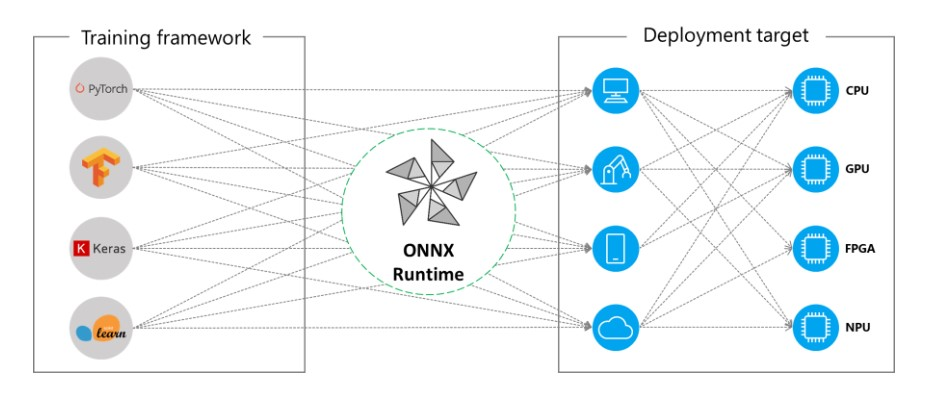
\includegraphics[width=10.5cm]{images/onnx.jpg}
\caption{ONNX Model environments \citep{onnx}}
\label{fig:onnxplot}
\end{center}
\end{figure}

\newpage
\section{RoboCup Soccer}
RoboCup is an internationally coordinated robotics competition with a focus on advancing artificial intelligence and robotics research. The ultimate goal of the soccer competition is to support the development of a team of fully autonomous humanoid robot soccer players that are capable of winning against the winner of the most recent soccer world cup, by the year 2050. Some of the characteristics of the RoboCup challenge is that it features a dynamic environment and distributed control performed in real time \citep{RoboCupObj}.\

There are various leagues which each emphasize different challenges that need to be addressed to achieve the ultimate RoboCup objective. Of particular interest is the RoboCup 3D Soccer Simulation League (3DSSL) as well as the Standard Platform League (SPL), which focuses on the software programming aspects of Nao robots.

\begin{figure}[h!]
    \centering
    \subfloat{{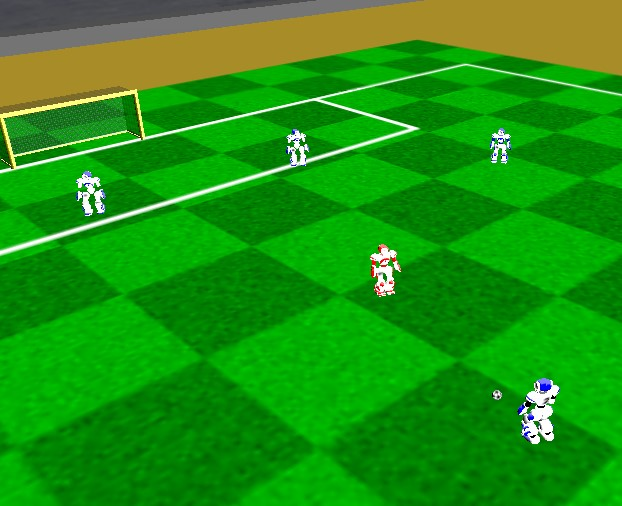
\includegraphics[height=5cm]{images/Robocup1.jpg}}}
    \qquad
    \subfloat{{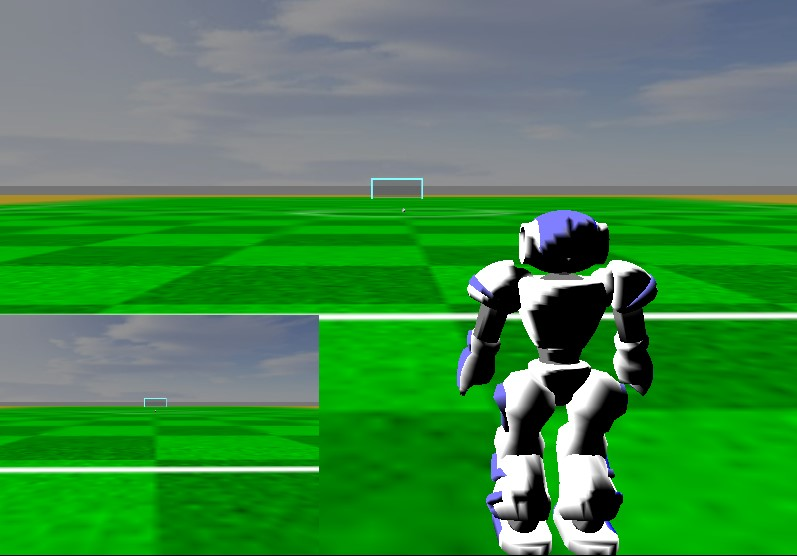
\includegraphics[height=5cm]{images/Robocup2.jpg}}}
    \caption{Simulated RoboCup Soccer (Left) and Simulated image perceptor (Right)}
\end{figure}

The position of the ball is crucial for determining appropriate agent behavior. At a close observation range the agent may need to kick the ball, in this case large errors will result in a miss-directed kick or perhaps a complete miss. At middle ranges the agent may attempt to block an opposition passing option and should position itself accordingly. At long ranges the agent may need to know what region of the field the ball is in so that an appropriate behavior is chosen. 

\subsection{RoboCup Soccer Simulator}

The RoboCup 3D Soccer Simulation League runs on a simulator known as the RoboCup Soccer Simulator Server (RCSSServer3d) which is developed using plugins to a generic physical multi-agent simulation platform, SimSpark. In the architecture of SimSpark, agents receive various sensor feedback from ``perceptors'' and take actions using ``effectors'' \citep{simspark}. In the current format of 3DSSL, a vision perceptor returns prepossessed visual data, in spherical coordinates, to each agent every three simulation cycles (60ms). Therefore in this league, computer vision is not within the scope of the challenge. The capabilities do however exist within the underlying SimSpark simulator to provide an image perceptor that produces rendered simulated camera images by enabling a plugin.

%\subsection{Nao}
%The Aldebaran Nao robot is the agent used in the 3DSSL and SPL RoboCup leagues. The robot has two cameras (figure \ref{fig:naocam}) placed on the head which can be rotated by a joint effector on the neck of the Nao (figure \ref{fig:naoneck}) to scan across the field. In the physical robot, the output image is given in a YUV colour space captured in 1280x960 at 30fps -- However it is possible to reduce the resolution of the camera and capture rate
%\citep{aldebaran}.
%
%\begin{figure}[h!]
%    \centering
%    \subfloat{{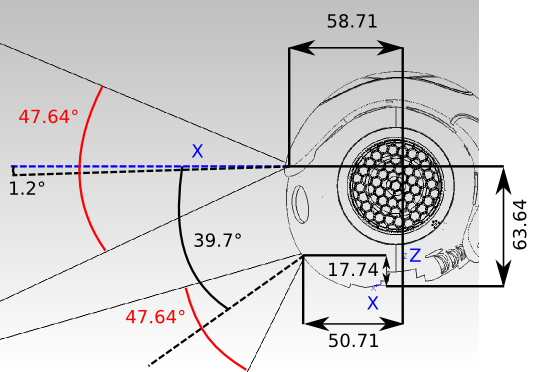
\includegraphics[height=4cm]{images/nao1.png}}}%
%    \subfloat{{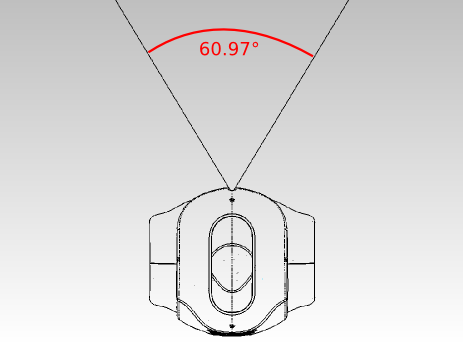
\includegraphics[height=4cm]{images/nao2.png}}}%
%    \caption{Nao Camera configuration \citep{aldebaran}}
%    \label{fig:naocam}
%\end{figure}
%
%\begin{figure}[h!]
%	\begin{center}
%	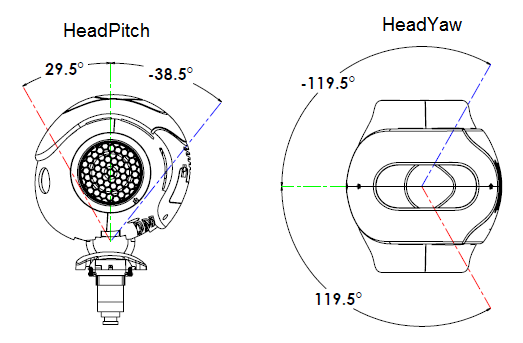
\includegraphics[width=7cm]{images/nao3.png}
%	\caption{Nao Neck effector \citep{aldebaran}}
%	\label{fig:naoneck}
%	\end{center}
%\end{figure}
%
%With the given camera configuration, the Nao has monocular vision. Further, due to the limited FOV of the cameras as well as the range limited yaw rotation of the Nao neck effector, there is a blind spot behind the robot. The two cameras can be accessed simultaneously. The Nao v6 features an intel Atom E3845 1.91Ghz Quad core CPU with 4GB DDR3 RAM \citep{naov6}.
%
%\subsection{Fat Proxy}
%Fat proxy is a sub league of the RoboCup Soccer simulation league which focuses on high level behavior by providing a common set of low level skills such as walking and kicking. The developers \cite{fatproxy} state, \textit{``To have simplified access to the simspark simulation, the Fat Proxy takes over all motor control of the simulated Nao robots. Agents control the robot with high level dash and kick commands. Anything else like getting up or focusing the head is done by the Fat Proxy''}. The tooling for this is useful as it can be used to isolate higher level behaviors from the low level skills of the robot.

\chapter{Related work}

In this section, a selection of published works that are related to ball detection  (Section 3.1) and tracking (Section 3.2) are considered. This overview lists some important approaches and results whilst keeping in mind the historical context. It is shown that recent approaches take advantage of fine tuning state-of-the-art CNN object detector architectures for transferring to their own problem domain as well as Kalman filtering for tracking.

\section{Ball detection}

The object detection space has significantly changed over time, with the most successful detectors being deep learning based. Using what is now considered a traditional approach, \cite{robovj} implement a Viola Jones based object detector that performs real-time ball detection with a focus on mobile robots in a Robocup soccer environment. They perform a edge detection proprocessing step which allows them to achieve a satisfactory color-independent result.

Attempting to apply more modern deep learning techniques to improve real-time ball localization, \cite{selfcnn} propose a novel CNN to localize multicolored, patterned balls for Robocup by formulating their approach as a regression problem. They develop an architecture that can process an entire image at once to avoid a sliding window approach by predicting Gaussians that correspond to probabilities of the ball location. They find their proposed model to be too large for their robot (over 2GB) but also find that reducing their model size leads to a poor performance. \cite{selfcnn} conclude, \textit{``Thus, either faster processors for robots are necessary (to run the bigger nets) or low classification rates at medium to high distances have to be accepted''}. Although the design was not successful, the single shot strategy is for real-time is widely adopted by state-of-the-art detectors such as YOLO.

Basing their work on the state-of-the-art single shot architecture, Tiny YOLO v3, \cite{robo} propose a real-time object detector which is fine tuned for RoboCup ball detection for the Nao v5 platform. The maximum reported speed is only 13 FPS. Synthetic transfer learning is successfully applied, which involves pretraining the network on a fully synthetic dataset. \cite{robocupdataset} evaluate several CNN models on an embedded RoboCup robotic system. They find that, for their RoboCup dataset, YOLOv4 Tiny performs the best in terms of AP@75 as well as for the small and medium images which points towards this model being the best for accurate ball detection. However, the detector fails to execute at real time speed on their Small Size League (SSL) platform, hence, the selection of the Mobile SSD architecture which does compute at real-time.

\section{Ball tracking}

In the ball tracking problem space, Kalman filtering has been successful and remains particularly popular. The approach of fusing measurements with a dynamic physics model allows noise attenuation as well as substep estimation for problems such as a parabolic trajectory or rolling with friction.

In order to establish the real-time capability of a non-linear Kalman filtering approach for use in RoboCup, \cite{robocuptrack} investigate tracking of ball trajectories using an unscented Kalman filter (UKF) and monocular vision. Although only the tracking problem is considered (manually processed images) the investigation confirms that, compared to a maximum likelihood estimator, UKF is feasible as a real-time tracker: \textit{``after half the time of flight the error is about 0.3m which we judge to be enough for playing soccer''}.

With a focus on RoboCup Middle Size League, \cite{3dparabola} consider the use of a extended Kalman filter (EKF) for real-time 3D Ball trajectory estimation using a single camera. In their research they propose applying a maximum Likelihood method to provide an initial estimate of the ball trajectory for the initialization which improves tracking of the ball.

\cite{golftrack} investigates real-time golf ball tracking by taking advantage of state-of-the-art CNN based object detection and Kalman filter based tracking -- with small object detection as a primary focus. They report: \textit{``most object detectors do not perform well on small object detection''} where is is explained that since most detectors are pretrained on datasets, such as MS COCO, where the size of the objects tend to be larger. The detectors: Faster R-CNN, SSD, YOLO v3, YOLO v4 as well as RefineDet are investigated, however, GPU compute is available. By cropping patches according to a prior location of the region of interest, the ball is made relatively “larger” which improves the accuracy.  

%%%%%%%%%%%%%%%%%%%%%%%%%%%%%%%%%%%%%%%%%%%%%%%%%%%%%%%%%%%%%%%%%%%%%%%%%%%%%%%%%%%%%%%%%%%%%%%%
\chapter{Problem Statement, Research Aims and Objectives}
\section{Problem Statement}

In RoboCup soccer most of the decision-making involves the position of the ball on the field. This affects factors such as how the players should move, when and where they should kick and how the goalkeeper should behave. In order to facilitate decision making, it is important to have an accurate understanding of the ball’s position and trajectory. In this research project, the interest lies in determining if it is feasible to accurately predict both the position and trajectory of the ball using a computer vision based system, with a neural network based approach utilized for tracking.

\section{Research Hypothesis}

Hybrid approaches to state estimation which fuse intuitive model based approaches with measured data are a promising technique for state estimation. It is hypothesized that a neural network assisted approach to Kalman filtering can outperform the traditional EKF method at tracking the trajectories of a kicked RoboCup soccer ball as measured by RMSE and speed, using a tracking-by-detection framework.

Modern object detection has significantly improved upon traditional approaches and various models promise reliable localization with real-time performance. Tracking-by-detection is a paradigm which takes advantage of this technological leap and can be paired with the popular Kalman filter for real-time robotics applications. It is hypothesized that a more recent key-point based modern object detection approach (NanoDet) can be to used to outperform popular anchor based method (Yolov4 Tiny) as well as the traditional Viola Jones detector for color-independent ball detection as measured by quality of inference using AP scores, at a realtime speed. 

\section{Research Aims and Questions}

The first aim of the research project will be to prepare a suitable real-time object detector trained on localizing the ball in a simulated Robocup soccer environment. A traditional architecture (Viola Jones detector) alongside a more modern anchor based detector (YOLOv4 Tiny) serve as a benchmark against a recent keypoint based approach (NanoDet). To motivate the selection of NanoDet, a selection of different pretrained CNN detector models which use different strategies such as single stage, anchor-based and key-point based approaches will be compared on inference speed and memory usage. Inference speed is evaluated on a laptop CPU as a compute constrained device. 

A significant challenge for object detection is the size of the ball which at distance is small in the image (as defined by COCO metrics). The ball used in RoboCup is also significantly white in colour and may be difficult to distinguish against the field markings, goals and Nao robots. The algorithm further needs to act in real-time since slow responses due to heavy computational load can result in delayed agent responses or leading to control inaccuracies and instability. The memory footprint of the architecture should also be considered in the context of embedded computing capacities, which can be improved using model quantization.

The principle questions which arise are:
\begin{itemize}
    \item Does the more recent keypoint based NanoDet detector outperform the proven anchor based Yolov4 Tiny and traditional Viola Jones detectors found in the related works, as measured by AP and latency, on a RoboCup ball tracking dataset? 
    \item Can a CNN object detector run at real-time on a modern mobile laptop CPU?
    \item Can pretraining on real images transfer to a simulated RoboCup environment?
    \item Does model quantization cause a noticeable performance degradation? 
\end{itemize}

The second aim of the research project will be to use the object detector to implement a tracking-by-detection framework based on neural aided Kalman filtering. Using ball telemetry from the robocup simulation as a ground truth and processing the associated visualization with the object detector, a tracker based on the KalmanNet approach can be trained. As a baseline, an extended Kalman filter can be implemented in a similar fashion to the Robocup trackers found in the related works. 

A significant challenge is the non-linearity of the trajectories due to rolling friction of the ball as well as the bouncing after the initial parabolic trajectory makes contact with the pitch. Such physics are not simply modeled in a standard linear Kalman filter. 

The principle questions which arise are:
\begin{itemize}
    \item In the context of the simulated RoboCup soccer environment, can a neural aided Kalman filter outperform a traditional EKF for:
    \begin{itemize}
    	\item Rolling kicks?
    	\item Lofted kicks?
	\end{itemize}
	\item Can a tracking-by-detection approach meet real-time performance requirements?
\end{itemize}

%%%%%%%%%%%%%%%%%%%%%%%%%%%%%%%%%%%%%%%%%%%%%%%%%%%%%%%%%%%%%%%%%%%%%%%%%%%%%%%%%%%%%%%%%%%%%%%%
\chapter{Research Methodology}

The methods used to investigate the proposed research topic can be conveniently separated into two distinct phases where the former focuses on object detection (Section 5.1) and the latter on tracking-by-detection (Section 5.2) using the previous result. 
%It is envisioned that the focus of the tracking will be (similar to the related work) focused on the trajectory of the kick investigated from the perspective of the kicker, and tested by against a set of randomized rolling and lofted kicks in a control RoboCup soccer environment. 

\section{Phase one: Object detector investigation}

In this phase, the training and performance of the Viola Jones, Yolov4 Tiny and NanoDet object detectors are considered. To justify the selection of NanoDet, an initial comparison of a variety of popular pretrained detectors will be evaluated on inference speed and memory utilization. The chosen object detectors are then fine-tuned on a representative data set, generated using the RoboCup simulator, and evaluated in order to determine which is the most promising as measured by AP, model size and latency. The AP score is evaluated on large, medium and small object sizes (as distinguished by the COCO guidelines) as well as against occlusion and background complexity. For the optimum architecture, the impact of model quantization is investigated.

\subsection{Dataset Generation}

The Robocup simulator contains an image perceptor plugin that can be enabled to produce perspective images at 25Hz (real-time). In this manner actual gameplay can be used to create representative data. 
%Although a ground truth ball position is available to be enabled, fatproxy does not directly support processing of the additional server message at this stage and will crash. The built in feedback which includes a small amount of noise can be used as an alternative if a work around (possibly using the visualizer) is not found. 
With some changes to the source code, ground truth bounding boxes can be automatically computed using a coordinate transform from the perceptor to the camera location followed by a correction from the wide angle image, in order to describe the ball center in image coordinates. The distance of the ball is used to compute the relative bounding box size.

Although the empty test environment is proposed for the kick tracking, including actual match images with features such as players, field markings and the goals in the background is prudent to ensure robustness and evaluate performance in a match environment where occlusion may also occur. Since the server provides an indication whether a ball is in the vision of an agent, actual match footage that can be classified as including a ball can be generated and then included in the dataset. It is noted however that a check for occlusion is not programmed into the server so the ball could be completely hidden, therefore some manual work will need to be done to remove such images and to seperate occluded images. The dataset will then need to be prepared according to the training requirements of the given model.

\subsection{Model selection}

The selection of the baseline Viola Jones and Yolov4 Tiny detectors follows on from the related works. NanoDet is proposed since it is a recent key-point based architecture with promising capabilities. To justify this choice, a set of various popular detectors will be evaluated on inference speed and memory utilization. The following pretrained models are selected from the ONNX model zoo \citep{modelzoo} as well as the investigation by \cite{comprehensive}: Faster-RCNN, YOLOv3, Tiny YOLOv3, SSD, Mobilenet SSD, YOLOX and NanoDet. The three investigated models are then fine-tuned to the RoboCup dataset and are evaluated and compared using AP, model size and latency (as measured in a single threaded application on a modern mobile laptop CPU).

The small scale of the ball (less than 32×32 pixels) at long range introduces a risk since it may cause difficulties in training and detection. Beyond network architecture and optimizations, the use of prior knowledge of the ball position to focus a window on the ball (as found in the related work) may boost the performance without large overhead. If this is unsuccessful, the kicking distance may be reduced to the maximum reliable range of the detector.

\subsection{Training}

Although it is possible in most cases to use pretrained model weights to significantly reduce training time -- the training of modern models can still require significant computational resources since typically it is desired to evaluate multiple different hyper-parameter combinations in order to optimize via a grid search. It is proposed to utilize the Wits Mathematical Sciences Cluster such that training can be done in parallel.  

A possible risk exists in using pretrained weights, since they are typically trained on real image datasets -- therefore domain transfer to a synthetic domain may fail to produce acceptable results. Further, most datasets used for pretraining feature few small scale object examples which may also be problematic for this application.

\subsection{Evaluation}
Models are all translated to a neutral ONNX format which serves two purposes here: Firstly, the runtime environment can be controlled with ONNX Runtime in order to limit the computational resources to single threaded execution. Secondly, it mimics practical model deployment as it is platform, device and training framework independent with support for multiple languages. 

\section{Phase two: Object tracking investigation}

In the next phase of the project, the tracking problem is considered by using the detector from phase one for tracking-by-detection. An EKF with a simple RoboCup world model (similar to the related work) will be implemented as a baseline tracker. A tracking dataset will need to be generated using the RoboCup simulator which will be used to train and optimize the neural assisted Kalman tracking framework. The trackers performances will then be compared on a test dataset with RMSE as a performance measure. Prior knowledge of the kick in the form of the initial velocity state is assumed.

\subsection{Dataset Generation}

To generate a tracking dataset, a series of randomized kicks are performed in order to capture image and ground truth position data that describes various trajectories. Kicks are performed from random locations on the training pitch in order to capture a variety of scenes. The tracking dataset can be produced by applying the object detector for inference which can be transformed into coordinates relative to the robot frame of reference. The simulator default sampling rate of 50hz will be applied for the ground truth. This rate is faster than the camera, which means that intermediate estimations (those without correction) will be evaluated.

\subsection{Training}
The neural assisted Kalman tracking will be based on the KalmanNet framework. By attempting to reproduce the results of the authors using the available implementation \cite{kalmangit}, it has been found that the implementation suffers significantly in-terms of training stability, initialization as well as GPU support (confirmed by others on issues page). In order to effectively train the model, it will be therefore required to investigate some architecture improvements and therefore  also familiarize with the chosen deep learning framework, PyTorch. Some architectural decisions have been noticed such as an unbounded Kalman gain as well as choice of non-descriptive input features should also be considered as areas for possible improvement.  

The use of this tracking framework introduces risk as the repository is still undergoing regular changes and is unreliable in its current state. However, it provides a starting point. In order to achieve the desired results, some exploring of the framework must be undertaken as well as some refactoring for this projects purposes. The results of these investigations can be returned to the original authors.

\subsection{Evaluation}

The tracking performance of the trackers will be evaluated and compared using the RMSE performance measure on the test dataset. The minimum real-time performance target will be to process images at atleast every 0.04 seconds (25 FPS).
%%%%%%%%%%%%%%%%%%%%%%%%%%%%%%%%%%%%%%%%%%%%%%%%%%%%%%%%%%%%%%%%%%%%%%%%%%%%%%%%%%%%%%%%%%%%%%%%
\chapter{Object detection investigation}

\section{Detection dataset}
The dataset is generated using various open source programs in the RoboCup soccer ecosystem as well as the Wits agent with a bespoke behavior. Half the images are acquired in a simulated match, the remainder are collected in a practice environment.

\subsection{Software environment}
The ball detection images are generated using the RoboCup match server rcssserver3d-0.7.3 which is built on the simspark-0.3.2 simulator. In the simulator, the ``agentSyncMode'' variable is changed to true to enable synchronized execution. In the match server: ``enableRealTimeMode'' is set to false, ``addNoise'' is set to false and an ``ImagePerceptor'' is added to the Nao model to enable rendered perspective images to be appended to the server messages sent to each agent.  

The Wits agent message parser is extended to include the vision messages which are received in a base64 string encoded format. Each image is stored as a .json file, for readability, which includes the image metadata such as the spherical coordinates of the ball (See figure \ref{fig:spherical}) (vertical angle, horizontal angle, distance) and the image size. 

\begin{figure}[h!]
\begin{center}
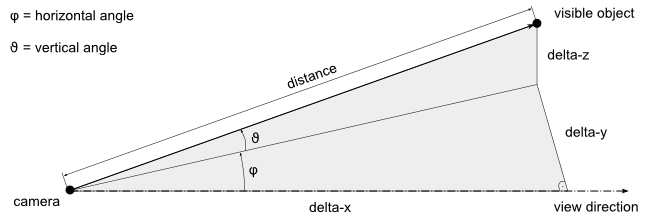
\includegraphics[width=12cm]{images/Vision_Perception.png}
\caption{RoboCup agent visual perception \citep{perceptors}}
\label{fig:spherical}
\end{center}
\end{figure}

Control of the agent is abstracted by using magmaFatProxy-1.2.2, which also needs to be extended to include the handling of vision messages.

\subsection{Preprocessing}

The images are decoded into an RGB array format that can be displayed, manipulated and stored using the Numpy and OpenCv Python libraries. In order to better understand the performance of each detector in the context of the image content, images are sorted into categories that classify ball visibility, occlusion, size as well as play mode. Occluded ball images must be manually separated.

From the spherical coordinates of the ball that are given by the match server relative to the center of the head of the Nao agent, it is possible to transform them to the position of the camera by converting the coordinates to a Cartesian axis, performing a translation and then returning the coordinate system to spherical. From the spherical coordinates at the camera position, with the known field of view of the lens being 58\textdegree, it is possible to use an ideal wide angle lens transformation to determine the bounding box center in image coordinates. This transformation is based on the ideal fish-eye lens model (See figure \ref{fig:blockd}) which is then extended to the two rotational axes using spherical geometry. The size of the bounding box is then determined based on the distance of the ball which has a known diameter of 8.4cm.

 \begin{figure}[h!]
\begin{center}
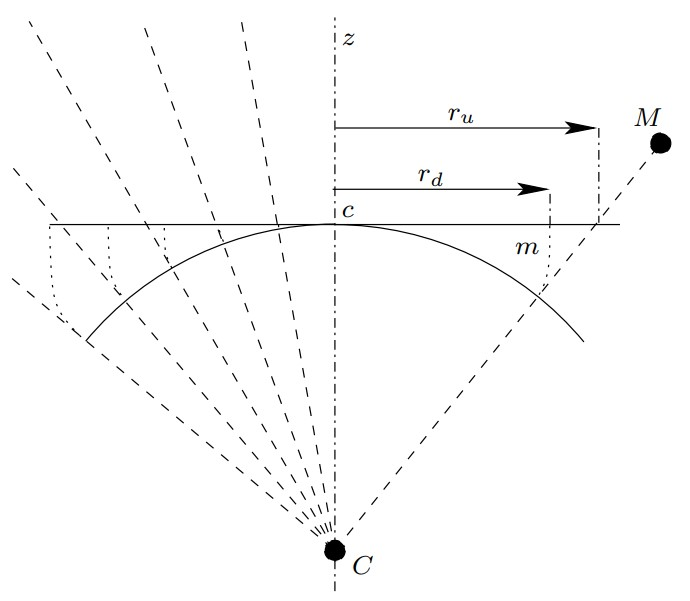
\includegraphics[width=7cm]{images/FOVmodel.jpg}
\caption{Ideal wide angle lens transformation \citep{wideangle} }
\label{fig:onnxplot}
\end{center}
\end{figure}

Although the described transformations can be automatically computed, using the simulator to produce perspective images for control purposes is outside of the typical usage of the simulator - it is found that in some agent initializations (approximately 1 in 5) that the synchronization of the produced images to the ground truth is between time steps. In these cases the data must be dropped, however, it requires a manual process of inspecting ground truth bounding boxes as a way of detecting bad initializations was not obvious. 

Each object detector expects the data-set to be presented in a certain structure with annotations in a specified format in order to facilitate dataloading. NanoDet utilizes the COCO format \citep{cocodataset} which is commonly used by recent detectors, whereas the VJ detector expects a bespoke format \citep{vjdataset}. Scripts are made to automate these conversions respectively from the .json formatted data. A 60:20:20 training, validation, test split is used for allocating data for the various downstream tasks.

\subsection{Data Exploration}
Stats

\section{Baseline detection}

\section{Proposed detection}

\section{Evaluation of detection}

\section{Optimization}

%%%%%%%%%%%%%%%%%%%%%%%%%%%%%%%%%%%%%%%%%%%%%%%%%%%%%%%%%%%%%%%%%%%%%%%%%%%%%%%%%%%%%%%%%%%%%%%%
\chapter{Object tracking investigation}

\section{Tracking dataset}
Once again, the dataset is generated using various open source programs in the RoboCup soccer ecosystem as well as the Wits agent with a bespoke behavior. Each kick is captured in a practice environment with a sequence of images at 25hz and the ground truth at 50Hz.

\subsection{Software environment}
The kick tracking data is also generated using the RoboCup match server rcssserver3d-0.7.3 and simspark-0.3.2 simulator using the same settings as before. Additionally, in the match server: a ball and agent ground truth perceptor is added to append global ball and agent positions to the server messages. The limit of the agent ``BeamEffector'' is changed to extend the beamable area of the agent into the opposition half.

Along side producing .json files for image with metadata as before, the Wits agent stores a .csv file for each kick sequence which captures, for each time step, ground positions as well as the agent transformation matrices from the Nao head coordinate system to the global coordinate system. The data is synchronized through the server time. 

Control of the agent is again abstracted by using magmaFatProxy-1.2.2, but needs to be extended to include the handling of vision messages. The agent beams to random

\subsection{preprocessing}
Outside field area
Instability

\section{Tracking dataset}
, ground truth perceptors are enabled 

\section{Baseline tracking}

\section{Proposed tracking}

\section{Evaluation of trackers}

%%%%%%%%%%%%%%%%%%%%%%%%%%%%%%%%%%%%%%%%%%%%%%%%%%%%%%%%%%%%%%%%%%%%%%%%%%%%%%%%%%%%%%%%%%%%%%%%
\chapter{Conclusion}

The aim of visual object tracking is to use a sequence of image frames to robustly estimate the motion state of a target object. This offers a versatile approach that is capable of acquiring an abundance of environmental information that can be used by robotic agents to perceive and interact with a dynamic environment in real-time. In this research report, the context of ball tracking in a simulated RoboCup soccer environment is considered. It has been proposed to take advantage of the progress of modern neural approaches to computer vision. Results from the popular problem space of object detection can be used for tracking by utilizing a tracking-by-detection framework. Correspondence can then be achieved through the the use of Kalman filtering which is a popular model based commonly used for state-estimation in the robotics domain. It is proposed to apply neural assisted Kalman filtering, which balances the ease of interpretation of a model-based approach and the ability to learn complex dynamics using neural networks. 

\section{Future work}

The natural continuation of this work would be to apply it to a physical robotic system to investigate how it generalizes to the real world with real physics as well as variations in scene and ball complexity.

A limitation of the approach used in this research is that a pipeline between detection and tracking is utilized rather than end-to-end training. Although, in this manner the performance of the detector can be better interrogated and extended to other classes that are independent of the tracking task. An approach which would train end-to-end, possibly utilizing a common backbone with different heads for each of the desired tasks, would result in better performances but at a cost of complexity and loss of intuition.

As a further extension of the real-time neural kalman filtering approach, the prediction of future time steps for significantly forward guesses might be considered, since the non-linearity of the systems investigated mean that using the partially known model for prediction alone would be inaccurate. This might be done by predicting future measurements on demand and fusing them to the partially known model.

%%%%%%%%%%%%%%%%%%%%%%%%%%%%%%%%%%%%%%%%%%%%%%%%%%%%%%%%%%%%%%%%%%%%%%%%%%%%%%%%%%%%%%%%%%%%%%%%
%\appendix
%\chapter{Appendix}\label{app:extra}
%Appendix A
%
%\section{Section 1}\label{app:whatis}
%Section 1

%%%%%%%%%%%%%%%%%%%%%%%%%%%%%%%%%%%%%%%%%%%%%%%%%%%%%%%%%%%%%%%%%%%%%%%%%%%%%%%%%%%%%%%%%%%%%%%%
%\chapter{Appendix}\label{app:extra}
%Appendix B

%\section{Section 1}\label{app:whatis}
%Section 1

%%%%%%%%%%%%%%%%%%%%%%%%%%%%%%%%%%%%%%%%%%%%%%%%%%%%%%%%%%%%%%%%%%%%%%%%%%%%%%%%%%%%%%%%%%%%%%%%
\bibliography{references}\addcontentsline{toc}{chapter}{References}
\end{document}
